\chapter{Stacks}

A \newterm{stack} is a linear data structure that only allows access at one end, called the \newterm{top}. 

Data comes off in the reverse order it went on: the last thing pushed onto the stack is the first thing popped off. This ordering is called \newterm{LIFO}, for ``last in, first out.'' 

You have already seen a stack in a previous workbook, even if it wasn't called one: the call stack from the Introduction to C chapter behaves exactly this way, with each function call pushing a new frame on top and returning popping it back off.

We can think of this like a stack of books: you can only access the book on top, and you can only see the cover of the top book. If you want to get to a book underneath, you have to remove the books above it first.
\begin{center}
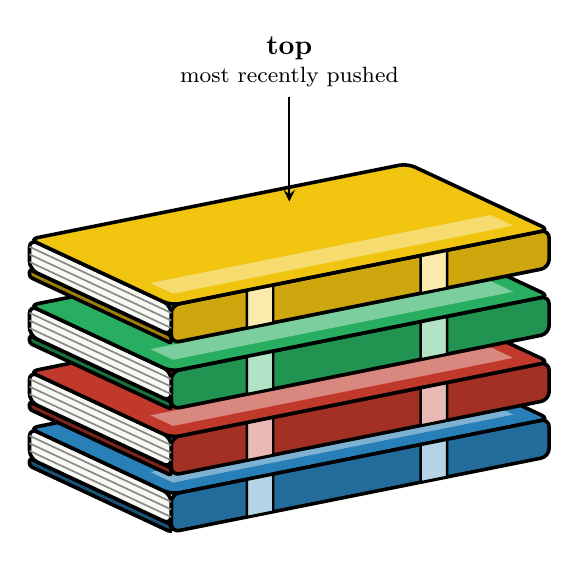
\begin{tikzpicture}[scale=1.2, line width=1.3pt]
  % Define colors for books and pages
  \definecolor{bookblue}{RGB}{41, 128, 185}
  \definecolor{bookred}{RGB}{192, 57, 43}
  \definecolor{bookgreen}{RGB}{39, 174, 96}
  \definecolor{bookyellow}{RGB}{241, 196, 15}
  \definecolor{pagescol}{RGB}{248, 248, 244}

  % Books stacked bottom to top: blue, red, green, yellow
  \foreach \col/\dy in {bookblue/0, bookred/0.6, bookgreen/1.3, bookyellow/2.0} {
    \begin{scope}[shift={(0,\dy)}]
      % spine (front edge), with two decorative bands
      \filldraw[draw=black, rounded corners=3pt, fill=\col!85!black] (0,0) -- (4,0.8) -- (4,1.2) -- (0,0.4) -- cycle;
      \filldraw[draw=black, line width=0.9pt, fill=\col!35!white] (0.80,0.16) -- (1.08,0.216) -- (1.08,0.616) -- (0.80,0.56) -- cycle;
      \filldraw[draw=black, line width=0.9pt, fill=\col!35!white] (2.64,0.528) -- (2.92,0.584) -- (2.92,0.984) -- (2.64,0.928) -- cycle;

      % back cover sliver (side edge, left side)
      \filldraw[draw=black, rounded corners=1pt, fill=\col!65!black] (0,0) -- (-1.5,0.7) -- (-1.5,0.78) -- (0,0.08) -- cycle;
      % pages (side edge, left side, with a few page lines)
      \filldraw[draw=black, rounded corners=3pt, fill=pagescol] (0,0.08) -- (-1.5,0.78) -- (-1.5,1.1) -- (0,0.4) -- cycle;
      \foreach \s in {0.25,0.5,0.75} {
        \draw[pagescol!55!black, line width=0.6pt] (0,{0.08+0.32*\s}) -- (-1.5,{0.78+0.32*\s});
      }

      % front cover (top face) with a gloss highlight streak
      \filldraw[draw=black, rounded corners=3pt, fill=\col] (0,0.4) -- (4,1.2) -- (2.5,1.9) -- (-1.5,1.1) -- cycle;
      \fill[white, opacity=0.4] (0.02,0.524) -- (3.62,1.244) -- (3.38,1.356) -- (-0.22,0.636) -- cycle;
    \end{scope}
  }

  % Arrow pointing to the most recently placed book (the top of the stack)
  \draw[-stealth, thick] (1.25,4.6) -- (1.25,3.5);
  \node[align=center, above] at (1.25,4.6) {\textbf{top}\\[-2pt]\footnotesize most recently pushed};

\end{tikzpicture}
\end{center}

Every stack, no matter how it is built underneath, supports the same handful of operations:

\begin{itemize}
    \item \texttt{push(value)} put a new value on top of the stack.
    \item \texttt{pop()} remove and return the value on top of the stack.
    \item \texttt{peek()} look at the value on top of the stack, without removing it.
    \item \texttt{isEmpty()} true if the stack has nothing in it.
\end{itemize}

Notice that we can only use the value on top of the stack, no matter how large it is.

We are going to build a stack two different ways: once backed by a fixed-size array, and once backed by the linked-list nodes from the previous chapter. Both give you \texttt{push}/\texttt{pop}/\texttt{peek}/\texttt{isEmpty}, but they make very different tradeoffs underneath.

\section{Array-Based Stack}

The simplest way to build a stack is on top of a plain array. We keep a fixed-size buffer and a single integer, \texttt{top}, that tracks the index of the top element. An empty stack is represented by \texttt{top == -1}.

\begin{minted}{cpp}
const int CAPACITY = 5;

struct ArrayStack {
    int data[CAPACITY];
    int top;   // index of the top element; -1 means empty
};
\end{minted}

\begin{center}
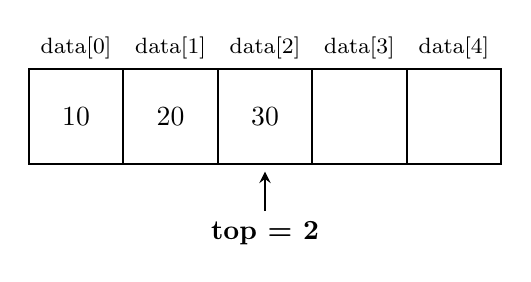
\begin{tikzpicture}[thick]
  \foreach \i/\v in {0/{}, 1/{}, 2/{}, 3/{}, 4/{}} {
    \draw (\i*1.2,0) rectangle ++(1.2,1.2);
  }
  \node at (0.6,0.6) {10};
  \node at (1.8,0.6) {20};
  \node at (3.0,0.6) {30};

  \draw[-stealth] (3.0,-0.6) -- (3.0,-0.1);
  \node[below] at (3.0,-0.6) {\textbf{top = 2}};

  \node[above] at (0.6,1.2) {\footnotesize data[0]};
  \node[above] at (1.8,1.2) {\footnotesize data[1]};
  \node[above] at (3.0,1.2) {\footnotesize data[2]};
  \node[above] at (4.2,1.2) {\footnotesize data[3]};
  \node[above] at (5.4,1.2) {\footnotesize data[4]};
\end{tikzpicture}
\end{center}

\texttt{push} and \texttt{pop} only ever touch the \texttt{top} index and whatever cell it points at, so both run in constant time, $O(1)$. The catch is \texttt{CAPACITY}: once the array is full, there is nowhere left to push, so a correct implementation has to check for and reject that case rather than writing past the end of the array.

\begin{minted}{cpp}
bool isEmpty(const ArrayStack& s) {
    return s.top == -1;
}

bool isFull(const ArrayStack& s) {
    return s.top == CAPACITY - 1;
}

void push(ArrayStack& s, int value) {
    // prevent pushing onto a full stack
    if (isFull(s)) {
        std::cout << "push(" << value << ") failed: stack overflow" << std::endl;
        return;
    }
    s.top++;
    s.data[s.top] = value;
}

int pop(ArrayStack& s) {
    // prevent popping from an empty stack
    if (isEmpty(s)) {
        std::cout << "pop() failed: stack underflow" << std::endl;
        return -1;
    }
    int value = s.data[s.top];
    s.top--;
    return value;
}
\end{minted}

Notice that \texttt{pop} does not actually erase \texttt{s.data[s.top]},
it just moves \texttt{top} down by one. The old value is still sitting
in the array, but nothing can reach it anymore, since every operation 
only ever looks at indices \texttt{0} through \texttt{top}. 

The full, 
runnable version of this file, including a \texttt{main()} that 
demonstrates both overflow and underflow, is in your digital resources. In this version, we added memory address output to demonstrate that shows how the array is a contiguous block.

\section{Linked-List Stack}

The array-based stack has one real weakness: \texttt{CAPACITY} is fixed at compile time. If you don't know in advance how much data you'll be pushing, you either waste memory reserving more than you need, or you risk overflow. A stack built on the \texttt{Node} type from the Linked Lists chapter has no limit, since it grows and shrinks on the heap as needed. The downside is that each element takes more memory, since it has to store a pointer to the next node.

\begin{minted}{cpp}
struct Node {
    int data;
    Node* next;
};

struct LinkedStack {
    Node* top;   // nullptr means empty
};
\end{minted}

Instead of an array index, \texttt{top} is now a pointer to the first node. Pushing means creating a new node whose \texttt{next} points at the old top, then moving \texttt{top} to the new node; popping is the reverse.

\begin{center}
\resizebox{0.85\textwidth}{!}{%
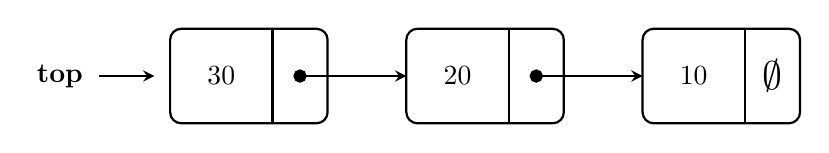
\begin{tikzpicture}[thick]
  \node at (-1.4,0.6) {\textbf{top}};
  \draw[-stealth] (-0.9,0.6) -- (-0.2,0.6);

  % top node (30)
  \draw[rounded corners=4pt] (0,0) rectangle (2,1.2);
  \draw (1.3,0) -- (1.3,1.2);
  \node at (0.65,0.6) {30};
  \filldraw (1.65,0.6) circle (2pt);
  \draw[-stealth] (1.65,0.6) -- (3,0.6);

  % middle node (20)
  \draw[rounded corners=4pt] (3,0) rectangle (5,1.2);
  \draw (4.3,0) -- (4.3,1.2);
  \node at (3.65,0.6) {20};
  \filldraw (4.65,0.6) circle (2pt);
  \draw[-stealth] (4.65,0.6) -- (6,0.6);

  % bottom node (10)
  \draw[rounded corners=4pt] (6,0) rectangle (8,1.2);
  \draw (7.3,0) -- (7.3,1.2);
  \node at (6.65,0.6) {10};
  \node at (7.65,0.6) {\Large $\emptyset$};
\end{tikzpicture}%
}
\end{center}

\begin{minted}{cpp}
bool isEmpty(const LinkedStack& s) {
    return s.top == nullptr;
}

void push(LinkedStack& s, int value) {
    Node* n = new Node();
    n->data = value;
    n->next = s.top;   // the new node points at the old top
    s.top = n;          // the new node becomes the top
}

int pop(LinkedStack& s) {
    if (isEmpty(s)) {
        std::cout << "pop() failed: stack underflow" << std::endl;
        return -1;
    }
    Node* oldTop = s.top;
    int value = oldTop->data;
    s.top = oldTop->next;
    delete oldTop;
    return value;
}
\end{minted}

Both \texttt{push} and \texttt{pop} still run in constant time (we will cover this in a future chapter), same as the array version, since neither one has to walk the list. But unlike the array version, \texttt{pop} here calls \texttt{delete} on the old top node; if it didn't, the node would sit on the heap forever.

The full version of this file is in your digital resource!

\section{Array vs. Linked: Which One?}

\begin{center}
\begin{tabular}{|l|l|l|}
\hline
 & \textbf{Array-Based} & \textbf{Linked-Based} \\
\hline
Max size & Fixed at compile time & Limited only by available memory \\
\hline
Memory per element & Just the value & Value + one pointer \\
\hline
\end{tabular}
\end{center}

If you know a safe upper bound on how much data you'll ever hold, the array version is the most efficient* choice. If you don't, the linked version is safer, since it will never overflow.
